\section{Changelog}
\begin{table}[H]
	\centering
	\begin{tabularx}{\linewidth}{l l X l}
		\toprule 
		\textbf{Date} & \textbf{Version} & \textbf{Changes} & \textbf{Autor} \\
		\midrule
		16.09.2020 & 0.1 & Erstfassung & Mike Schmid \\
		22.09.2020 & 0.2 & Korrekturen & Mike Schmid \\
		29.09.2020 & 0.3 & Anpassungen Risikoanalyse & Mike Schmid \\
		08.11.2020 & 0.4 & Anpassung Iterationen und Meilensteine & Mike Schmid \\
		15.12.2020 & 0.5 & Korrektur Abgabedatum vom 08.11 auf den 15.01.2021 & Mike Schmid \\
		\multirow{2}{*}{03.01.2021} & \multirow{2}{*}{1.0} & \multirow{2}{=}{Finalisieren der Projektdokumentation} & Janik Schlatter \& \\
		& & & Mike Schmid\\
		\bottomrule 
	\end{tabularx} 
	\caption{Changelog Projektmanagement} 
\end{table}

\clearpage

\section{Einführung} 

\subsection*{Zweck}
Dieser Teil der Dokumentation beschreibt die Projektplanung und bietet 
eine Übersicht über den Verlauf der Bachelorarbeit "Mobile Fingerprinting". 
Im Detail wird auf die Planung, Organisation und den Projektaufbau und -ablauf 
eingegangen.

\subsection*{Gültigkeit}
Der Gültigkeitsbereich ist auf die Dauer der Durchführung der Bachelorarbeit 
"Mobile Fingerprinting" im Herbstsemester 2020 an der Fachhochschule OST 
beschränkt.

\subsection*{Sprache}
Die allgemeine Projektsprache (Dokumentation, Protokolle, etc.) wird in 
deutscher Schriftsprache verfasst. 
Der Code, das GitHub-Repository und die Versionskontrolle wird in 
englischer Sprache geschrieben.

\subsection*{Referenzen}
Alle Dokumente werden auf dem GitHub-Repository 
\footnote{
	\hyperref[Repository]{
		https://github.com/EkoGuandor229/BA-MobileFingerprinting
	}
} abgelegt und verwaltet.


\subsection*{Vorarbeit}
Im Vorjahr wurde eine Studienarbeit mit dem Namen "Passenger Tracking" 
durchgeführt, die versucht hat, mittels Machine Learning ein Programm 
zu entwickeln, welches Passagiere im öffentlichen Verkehr anhand der 
von den Mobilgeräten ausgesendeten Probe-Requests erkennen kann. 
Dazu wurden den Studierenden 170 Millionen gesammelte WLAN-Daten vom 
Industriepartner für das Training des Algorithmus zur Verfügung gestellt. 
Der Prototyp konnte die Anzahl Geräte in einem Bus mittels eines Clustering 
Algorithmus mit durchschnittlich 94\% Genauigkeit ermitteln.

Diese Bachelorarbeit soll sich im Gegensatz zur Vorarbeit direkt 
mit dem Verhalten der Mobilgeräte auseinandersetzen. 
Wie wird die MAC-Address-Randomisierung von verschiedenen 
Herstellern mit unterschiedlichen Betriebssystemversionen durchgeführt 
und wie kann man die Unterschiede dafür nutzen, ein Gerät eindeutig zu 
identifizieren und zu verfolgen?

\clearpage

\section{Projektübersicht
\label{Projektübersicht}} 
Auszug aus der Aufgabenstellung:\newline
"Smartphones senden regelmässig WLAN-Probe-Requests, 
um Access Points zu finden. 
In der Vergangenheit konnte durch das Auslesen der MAC-Adresse aus 
diesen Requests ein Gerät über längere Zeit verfolgt werden.

Seit einigen Jahren wird diese Verfolgung durch die Verwendung von
anonymi-sierten MAC-Adressen erschwert. 
Weitere Datenfelder in diesen Requests können für das Tracken aber
weiterhin von Nutzen sein.

In einer früheren Arbeit wurde anhand bestehender Daten eines 
Industriepartners ein Top-Down-Ansatz mittels Machine Learning erarbeitet,
der aber nicht zu genügend genauen Resultaten führte."

\subsection*{Zweck und Ziel}
Das Verschleiern von MAC-Adressen durch Randomisierung ist seit einigen 
Jahren eine gängige Praxis, um die Verfolgung von Benutzern durch 
Organisationen oder Einzelpersonen zu verhindern. Dabei spielt es keine 
Rolle, ob die Verfolgung für statistische Zwecke, für personalisierte 
Werbung oder mit böswilligen Absichten geschieht.

Diese Arbeit befasst sich damit, wie diese Verschleierung von einzelnen 
Anbietern von Mobilgeräten durchgeführt wird und ob sich die Umsetzung
in unterschiedlichen Betriebssystemversionen unterscheidet. 
Durch Experimente soll herausgefunden werden, wie die Verschleierung 
in modernen Geräten in verschiedenen Versionen der Betriebssysteme 
umgesetzt wird. Weiterhin soll ein Prototyp entwickelt werden, 
der die gewonnenen Erkenntnisse umsetzt und die Verfolgung eines 
Gerätes über mehrere WLAN-Access-Points ermöglicht. Die für das 
Training und die Verifizierung des Prototyps benötigten Daten sollen 
in den Experimenten erfasst und aufbereitet werden.

\clearpage

\subsection*{Lieferumfang}
\begin{itemize}
	\item Auswertung, wie die Randomisierung bei MAC-Adressen von
	verschiedenen Anbietern, Mobilgeräten und Betriebssystemen umgesetzt
	wird und welche weiteren Eigenschaften/Attribute von Probe-Requests 
	sonst noch zur Erkennung verwendet werden können.
	\item Proof-of-Concept Prototyp, der die Verfolgung eines 
	zuvor kategorisierten Mobilgerätes (potentiell über mehrere 
	WLAN-Access-Points)	ermöglicht, falls möglich.
	\item Source-Code des Prototyps
	\item Protokolle, Dokumentation und gewonnene Daten der Experimente
	\item Sitzungsprotokolle
	\item Bericht der Bachelorarbeit gem. den Vorgaben der Hochschule 
	und des Projektbetreuers
	\item Abstract der Arbeit für das Online-Tool der Hochschule
	\item Plakat mit den wichtigsten Eckpunkten für die 
	Bachelorarbeitspräsentation
	\item Eigenständigkeitserklärung
	\item Einverständniserklärung für die Publikation
	\item Vereinbarung über Urheber- und Nutzungsrechte
\end{itemize} 

\subsection*{Annahmen und Einschränkungen}
Für die Bachelorarbeit sind 12 ECTS vorgesehen. 
Pro Person fällt somit ein Arbeitsaufwand von 360 Stunden, 
für die Arbeit gesamthaft 720 Stunden an.
Die Bachelorarbeit muss bis zum 15.01.2021 abgegeben werden.

\clearpage

\section{Projektorganisation 
\label{Projektorganisation}}

\subsection*{Projektmitglieder}
\begin{table}[H]
	\centering
	\begin{tabularx}{\linewidth}{X X}
		Mike Schmid & Janik Schlatter \\
		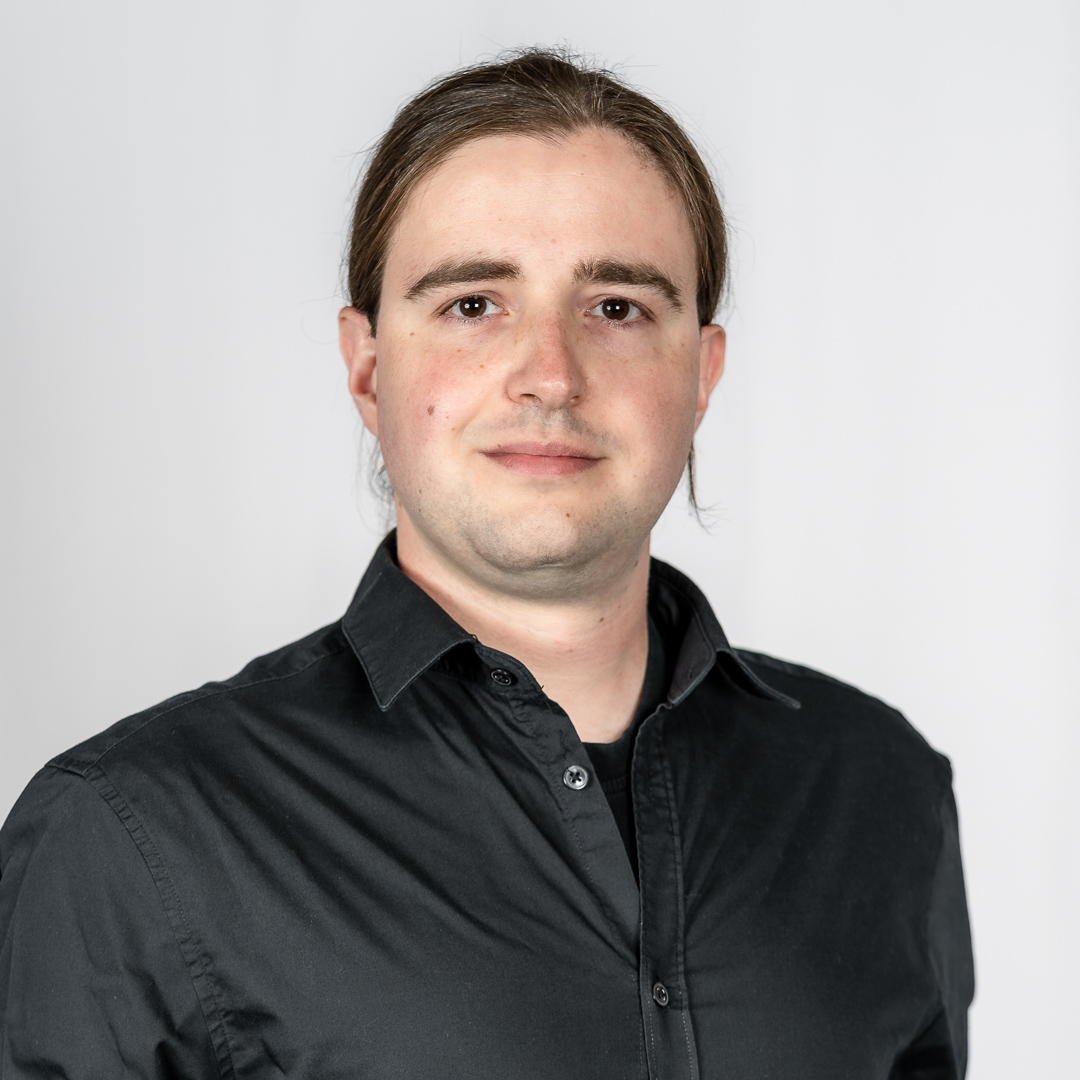
\includegraphics[width=0.75\linewidth]{Portrait_Schmid_Mike-2.jpg}
		&
		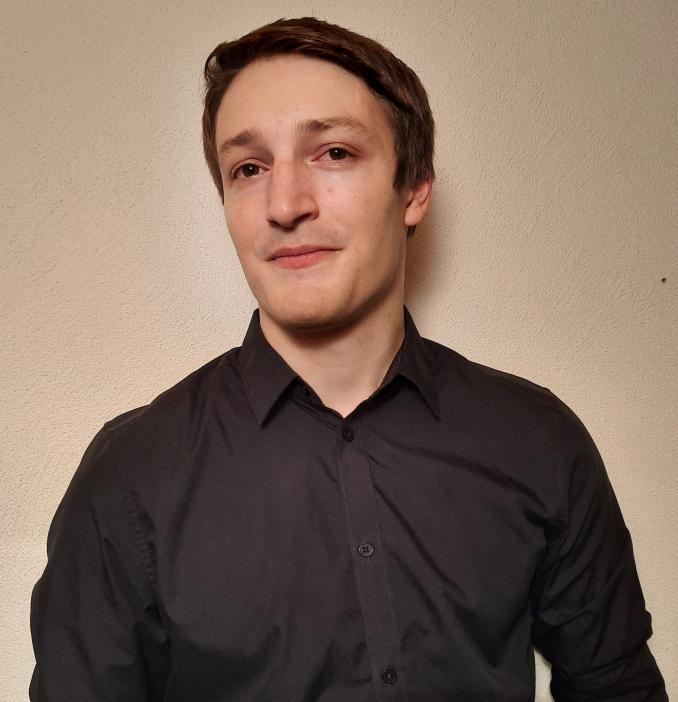
\includegraphics[width=0.73\linewidth]{Portrait_Janik.png}
	\end{tabularx} 
\end{table}

\subsection*{Externe Schnittstellen}
\begin{table}[H]
	\centering
	\begin{tabularx}{\linewidth}{| X | X | X |}
		\hline
		Prof. Beat Stettler & Martin Willi & Claudio Fuchs \\
		Betreuer & Experte & Gegenleser\\
		\hline
	\end{tabularx} 
\end{table}

\clearpage

\section{Management 
\label{Management}} 

\subsection*{Eckdaten}
Die Bachelorarbeit startet am 14.09.2020 und endet am 15.01.2021. 
In diesem Zeitraum werden die 360 Stunden Arbeit der einzelnen 
Projektmitglieder erbracht.
Zu Beginn der Arbeit wurde davon ausgegangen, dass die Arbeit in der 
zweiten Januarwoche am 08.01.2021 abgegeben werden muss. 
Die Arbeit wurde auf dieses Abgabedatum hin geplant und durchgeführt.
Die zusätzliche Woche wird als Reservezeit für allfällige Nachbesserungen 
betrachtet.

Gesamthaft stehen in diesem Zeitraum - bis am 08.01.2021 - 17 Wochen zur Verfügung, 
was in einem Wochendurchschnitt von 21.18 Stunden pro Person entspricht. 
Um die Planung zu vereinfachen, wurde die zu leistende Zeit auf 21h/Person 
und Woche festgelegt. 
Die Übrigen drei Stunden werden in der Abschlussphase verwendet, 
um die Dokumentation fertigzustellen. 

\begin{table}[H]
	\centering
	\begin{tabularx}{\linewidth}{X l}
		\toprule 
		Projektdauer & 17 Wochen  \\
		Anzahl Projektmitglieder & 2 \\
		Arbeitszeit für Projekt pro Woche und Mitglied & 21 Stunden \\
		Total Stunden pro Mitglied & 360 Stunden \\
		Arbeitsstunden Total & 720 Stunden \\
		Projektstart & 14.09.2020 \\
		Projektende (geplant) & 08.01.2021 \\
		\bottomrule 
	\end{tabularx} 
\end{table}

Die folgenden Absenzen sind beim Projektbeginn bekannt und eingeplant:
\begin{table}[H]
	\centering
	\begin{tabularx}{\linewidth}{X l l}
		\toprule 
		\textbf{Mitglied} & \textbf{Von} & \textbf{Bis} \\
		\midrule
		Janik Schlatter & 22.10.2020 & 30.10.2020 \\
		Beide & 24.12.2020 & 27.12.2020 \\
		\bottomrule 
	\end{tabularx}  
\end{table}
Jedes Projektmitglied ist selbst dafür verantwortlich, 
die Abwesenheiten entsprechend zu kompensieren.

\clearpage

\subsection*{Zeitliche Planung}
Die 17 Wochen des Projekts werden in vier Phasen unterteilt: 
\begin{itemize}
	\item Initialisierung
	\item Recherche
	\item Experimente, Implementation \& Evaluation
	\item Abschluss
\end{itemize}
In der Abbildung~\ref{figure:Projektphasen} sind die einzelnen 
Phasen ersichtlich. 
Da in der dritten Phase die Implementation davon abhängt, 
dass durch die Experimente statistisch relevante Erkenntnisse gewonnen werden, 
welche für einen Prototypen genutzt werden können, 
vereinheitlicht die dritte Phase die Experimente, 
Evaluation und das Prototyping. 

\begin{figure}[h!]
	\centering
	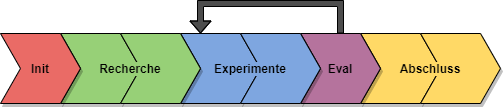
\includegraphics[width=1\linewidth]{ProjektPhasen.png}
	\caption{Projektphasen
	\label{figure:Projektphasen}}
\end{figure}
	
\subsection*{Iterationen}
Eine Iteration beträgt in der zweiten Phase zwei
und in der dritten Phase drei Wochen. 
Jeweils im nächsten Meeting nach einer Iteration werden die gewonnenen 
Erkenntnisse und das weitere Vorgehen besprochen. 
In der Tabelle~\ref{table:Projektiterationen} sind die einzelnen 
Iterationen und deren Tätigkeiten beschrieben.

\begin{landscape}
	\begin{table}[H]
		\centering
		\begin{tabularx}{\linewidth}{l X l l}
			\toprule 
			\textbf{Iteration} & \textbf{Inhalt} & \textbf{Start} & \textbf{Ende} \\
			\midrule
			Initialisierung & Projektstart und Kick-Off Meeting & 14.09.2020 & 20.09.2020 \\
			\midrule
			Research & 
			Wissensaufbau, Dokumentenstudium, Paperstudium und vorbereiten erstes Experiment &
			21.09.2020 &
			04.10.2020 \\
			\midrule
			Experiment 1 & Planen, durchführen und auswerten erstes Experiment & 05.10.2020 & 25.10.2020 \\
			Experiment 2 & Planen, durchführen und auswerten zweites Experiment & 26.10.2020 & 29.11.2020 \\
			Prototype 1 & Implementation erster Prototyp für Klassifizierung eines Mobilgeräts & 30.11.2020 & 13.12.2020 \\
			Experiment/Prototype & Iterativ weitere Experimente oder Weiterentwicklung Prototyp & 14.12.2020 & 27.12.2020 \\
			\midrule
			Abschluss & Fertigstellen Dokumentation, Aufbereiten der Ergebnisse für Abgabe & 28.12.2020 & 08.01.2021 \\
			\bottomrule 
		\end{tabularx} 
		\caption{Projektiterationen
		\label{table:Projektiterationen}} 
	\end{table}
\end{landscape}

\clearpage

\subsection*{Meilensteine}
In der Bachelorarbeit wurden Meilensteine gemäss der 
Tabelle~\ref{table:Meilensteine} festgelegt.
\begin{table}[H]
	\centering
	\begin{tabularx}{\linewidth}{l X l l}
		\toprule 
		\textbf{Meilenstein} & \textbf{Beschreibung} & \textbf{Termin} & \textbf{Aufwand} \\
		\midrule
		M1 & Projektplan & 20.09.2020 & 42h (1 Woche) \\
		M2 & Recherche & 04.10.2020 & 84h (2 Wochen) \\
		M3 & Experimente 1 \& 2 & 29.11.2020 & 336h (8 Wochen) \\
		M4 & Prototyp 1 & 29.11.2020 & 84h (2 Wochen) \\
		M5 & Experiment 3 \& Prototyp 2 & 27.12.2020 & 84h (2 Wochen) \\
		M6 & Schlussabgabe & 08.01.2021 & 84h (2 Wochen) \\
		\bottomrule 
	\end{tabularx} 
	\caption{Meilensteine
	\label{table:Meilensteine}} 
\end{table}

\subsection*{Meetings und Informationsfluss}
Die Projektmitglieder haben drei Tage - Dienstag, Mittwoch und Donnerstag -
an denen sie jeweils gemeinsam an der Bachelorarbeit arbeiten. 
An jedem Tag stehen mindestens sechs Lektionen für die Bearbeitung der 
anstehenden Arbeiten zur Verfügung.

Besprechungen zwischen den Projektteilnehmern und dem Betreuer finden
einmal alle ein bis zwei Wochen statt, um sich über den Stand der Arbeit
und gewonnene Erkenntnisse auszutauschen. 
Meetings können vor Ort an der Hochschule in einem dafür geeigneten Raum 
oder über Microsoft Teams durchgeführt werden.

\fbox{
	\begin{minipage}{\linewidth}
	Die in den Sitzungen besprochenen Pendenzen und Entscheidungen 
	können aus den Sitzungsprotokollen entnommen werden die sich im 
	Anhang~\ref{meetings} befinden.
	\end{minipage}
}

\clearpage

\section{Risikomanagement
\label{Risikomanagement}}
Mögliche Risiken wurden während der Bachelorarbeit fortlaufend evaluiert 
und angepasst, um auf unvorhergesehene Ereignisse möglichst verhältnismässig 
reagieren zu können.

\subsection*{Risiken}
Eine Risikoanalyse mit gewichtetem Schaden und Informationen, 
wie mit diesen Risiken umgegangen wird, 
ist im Dokument «TechnischeRisiken.xlsx» zu finden. 
Die Abbildung~\ref{figure:Risikomatrix} zeigt die Risikomatrix zum Beginn
der Bachelorarbeit am 14.09.2020.

\begin{figure}[h!]
	\centering
	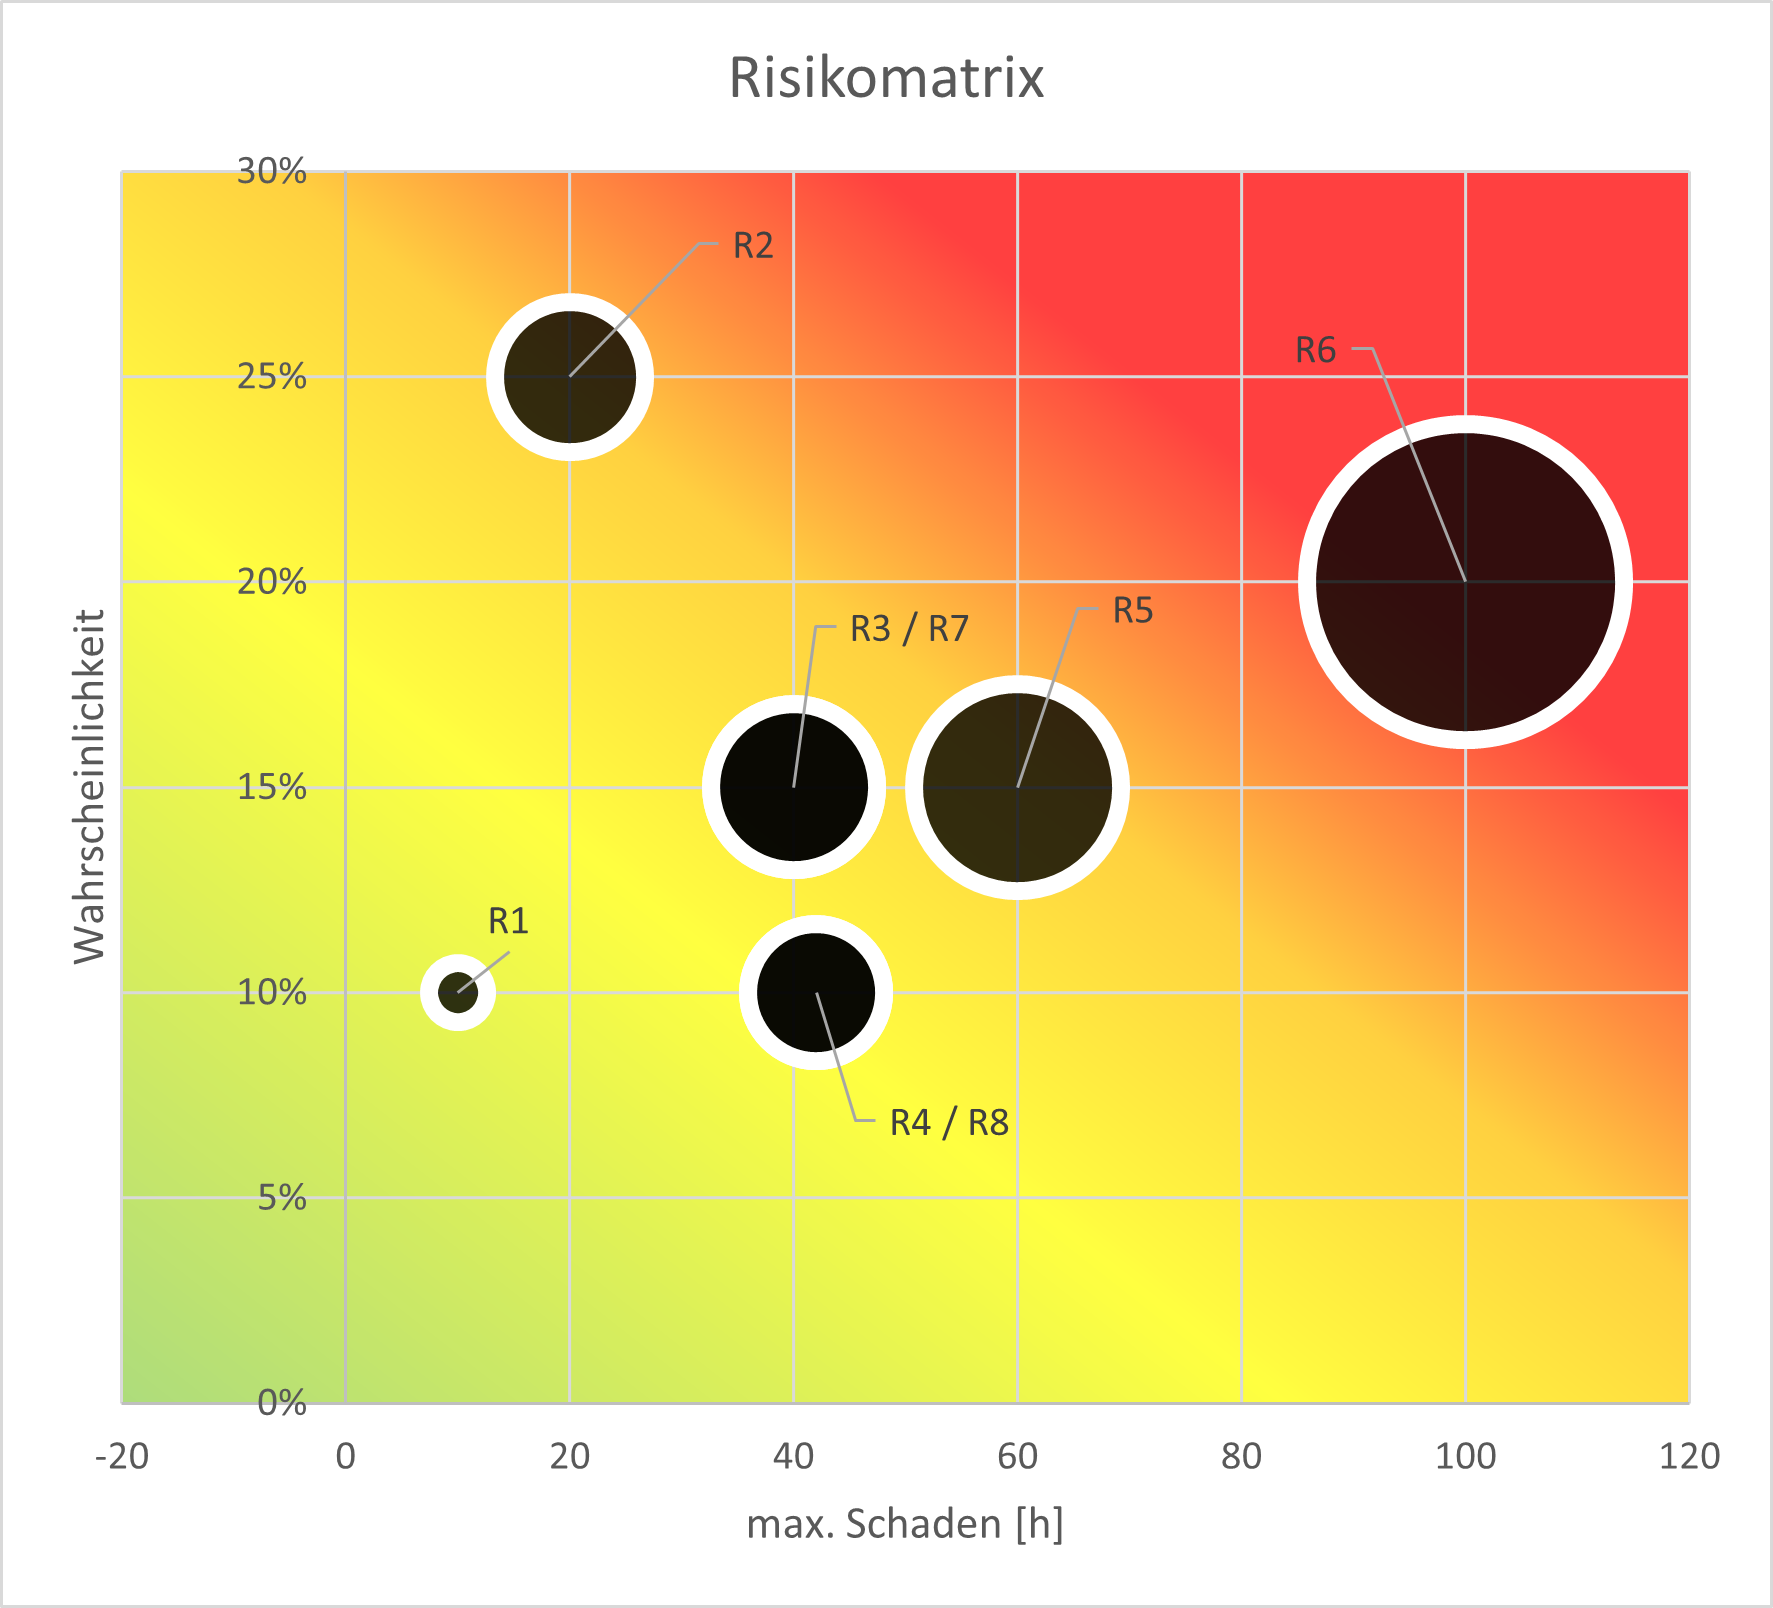
\includegraphics[width=1\linewidth]{RisikoMatrix.png}
	\caption{Risikomatrix, die Grösse der Blasen entspricht dem gewichteten Schaden
	\label{figure:Risikomatrix}}
\end{figure}

\begin{table}[H]
	\centering
	\begin{tabularx}{\linewidth}{| l | X | l | X |}
		\hline
		R1 & Testgeräte & R5 & Format Versuchsdaten \\
		\hline
		R2 & Testvorbereitung & R6 & Gerätemerkmale \\
		\hline
		R3 & Testdurchführung & R7 & Geräteverhalten \\
		\hline
		R4 & Testauswertung & R8 & Hardwareverhalten \\		
		\hline 
	\end{tabularx} 
	\caption{Risiken der Risikomatrix
	\label{table:RisikenMatrix}} 
\end{table}

\clearpage 

\subsection*{Risikoentwicklung und Risikoüberwachung}
Nachfolgend sind in den Tabellen~\ref{table:AenderungRisikoAnalyse}
die Änderungen der Risiken im Verlauf der Bachelorarbeit dokumentiert.

\begin{table}[h!]
	\centering
	\begin{tabularx}{\linewidth}{l l X}
		\toprule 
		\textbf{Risiko} & \textbf{Änderung} & \textbf{Begründung} \\
		\midrule
		R6 Gerätemerkmale & Neues Risiko & Hinzufügen Hardwarerisiken \\
		\midrule
		R7 Geräteverhalten & Neues Risiko & Hinzufügen Hardwarerisiken \\
		\midrule 
		R8 Geräteverhalten & Neues Risiko & Hinzufügen Hardwarerisiken \\ 
		\midrule
		\multirow{2}{*}{R1 Testgeräte} & Schaden: 10h $\rightarrow$ 5h & \multirow{2}{=}{Eingetretenes Risiko} \\
		& Wahrscheinlichkeit: 10\% $\rightarrow$ 5\% & \\
		\midrule
		\multirow{4}{*}{R2 Testvorbereitung} &  &  \multirow{4}{=}{Vorbeugung durch Absprache mit Betreuer} \\
		& Schaden 20h $\rightarrow$ 10h & \\
		& Wahrscheinlichkeit: 25\% $\rightarrow$ 5\% & \\
		& & \\
		\midrule 
		\multirow{2}{*}{R3 Testdurchführung} & Schaden: 40h $\rightarrow$ 30h & \multirow{2}{=}{Eingetretenes Risiko} \\
		& Wahrscheinlichkeit: 15\% $\rightarrow$ 10\% & \\
		\midrule
		R4 Testauswertung & Wahrscheinlichkeit: 10\% $\rightarrow$ 5\% & Vorbeugung \\
		\midrule 
		R5 Format  & \multirow{2}{*}{Wahrscheinlichkeit: 15\% $\rightarrow$ 5\%} & \multirow{2}{*}{Vorbeugung} \\
		Versuchsdaten& & \\
		\midrule  
		R6 Gerätemerkmale & Schaden: 100h $\rightarrow$ 80h & Eingetretenes Risiko \\
		\midrule 
		R7 Geräteverhalten & Schaden: 40h $\rightarrow$ 30h & Eingetretenes Risiko \\
		\bottomrule 
	\end{tabularx} 
	\caption{Änderungen der Risikoanalyse
	\label{table:AenderungRisikoAnalyse}} 
\end{table}

\clearpage 

\subsection*{Eingetretene Risiken}
In der Aufzählung~\ref{figure:EingetreteneRisiken} sind die eingetretenen 
Risiken aufgeführt. 
Risiken aus der Analyse, die nicht in der Aufzählung vorkommen, 
sind im Projektverlauf nicht eingetreten oder konnten durch vorbeugende 
Massnahmen verhindert werden.

\begin{figure}[h!]
	\begin{itemize}
	\item R1 - Testgeräte. Die vorhandene Hardware konnte nicht zur 
	Aufzeichnung der Probe-Requests verwendet werden. Es wurde 
	Frühzeitig ein Ersatzlaptop organisiert. Zeitaufwand: ca. 2 Stunden 
	\item R3 - Testdurchführung. Es mussten zwei zusätzliche Messungen 
	durchgeführt werden, da der ursprüngliche Testplan die benötigten 
	Daten nicht abdeckte. Zeitaufwand: ca. 4 Stunden
	\item R6 - Gerätemerkmale. Die iOS-Geräte liefern zu wenige 
	eindeutige Merkmale, als dass damit ein Fingerprinting durchgeführt
	werden könnte. Es wird in der Dokumentation darauf eingegangen, 
	sonst aber keine Massnahmen ergriffen.
	\item R7 - Geräteverhalten. Die Samsung Galaxy S8 verhalten sich im 
	Timing alle unterschiedlich. Die iPhone X haben unterschiede im Verhalten.
	In der Analyse wurde auf die Unterschiede eingegangen. Kein Zeitverlust.
	\end{itemize}
	\caption{Eingetretene Risiken
	\label{figure:EingetreteneRisiken}}
\end{figure}

\clearpage

\section{Arbeitspakete}
Die Arbeitspakete in der Bachelorarbeit werden mittels eines Excel-Dokuments 
verwaltet. Zu Beginn eines Meilensteins werden, wo sinnvoll, Arbeitspakete
erfasst, deren Zeitaufwand geschätzt und zugeteilt. 

Ein Arbeitspaket beinhaltet:
\begin{itemize}
	\item Titel
	\item Beschreibung
	\item Sub-Tasks
	\item Definition of Done 
	\item Geschätzter Aufwand
	\item Tatsächlich benötigter Aufwand
\end{itemize}

\subsection*{Auswertung der Arbeitspakete}

\subsubsection*{Phase 1: Initialisierung}
\begin{figure}[h!]
	\centering
	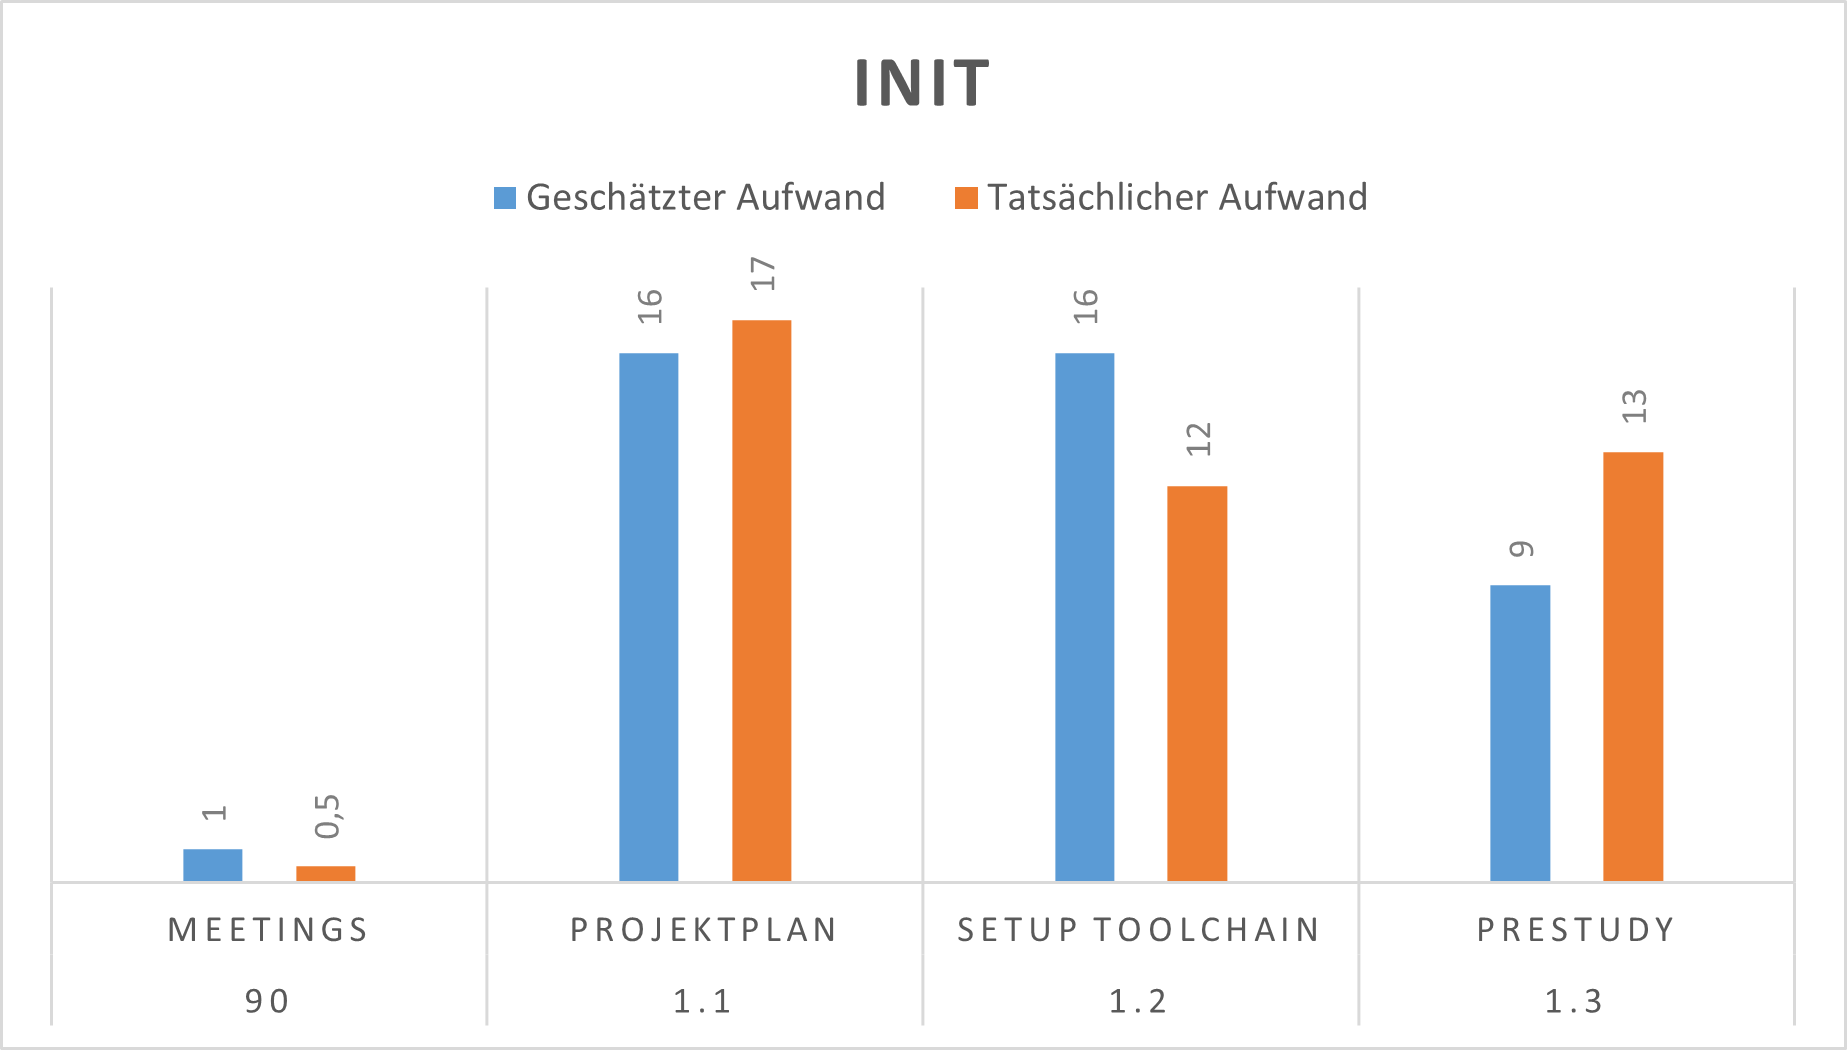
\includegraphics[width=1\linewidth]{Projectmanagement/Init_Auswertung.png}
	\caption{Auswertung der Arbeitspakete in der Initialisierungsphase
	\label{figure:initevaluation}}
\end{figure}

Geplanter Aufwand: $42$ Stunden. \\
Tatsächlicher Aufwand: $42.5$ Stunden.

\clearpage 


\subsubsection*{Phase 2: Recherche}
\begin{figure}[h!]
	\centering
	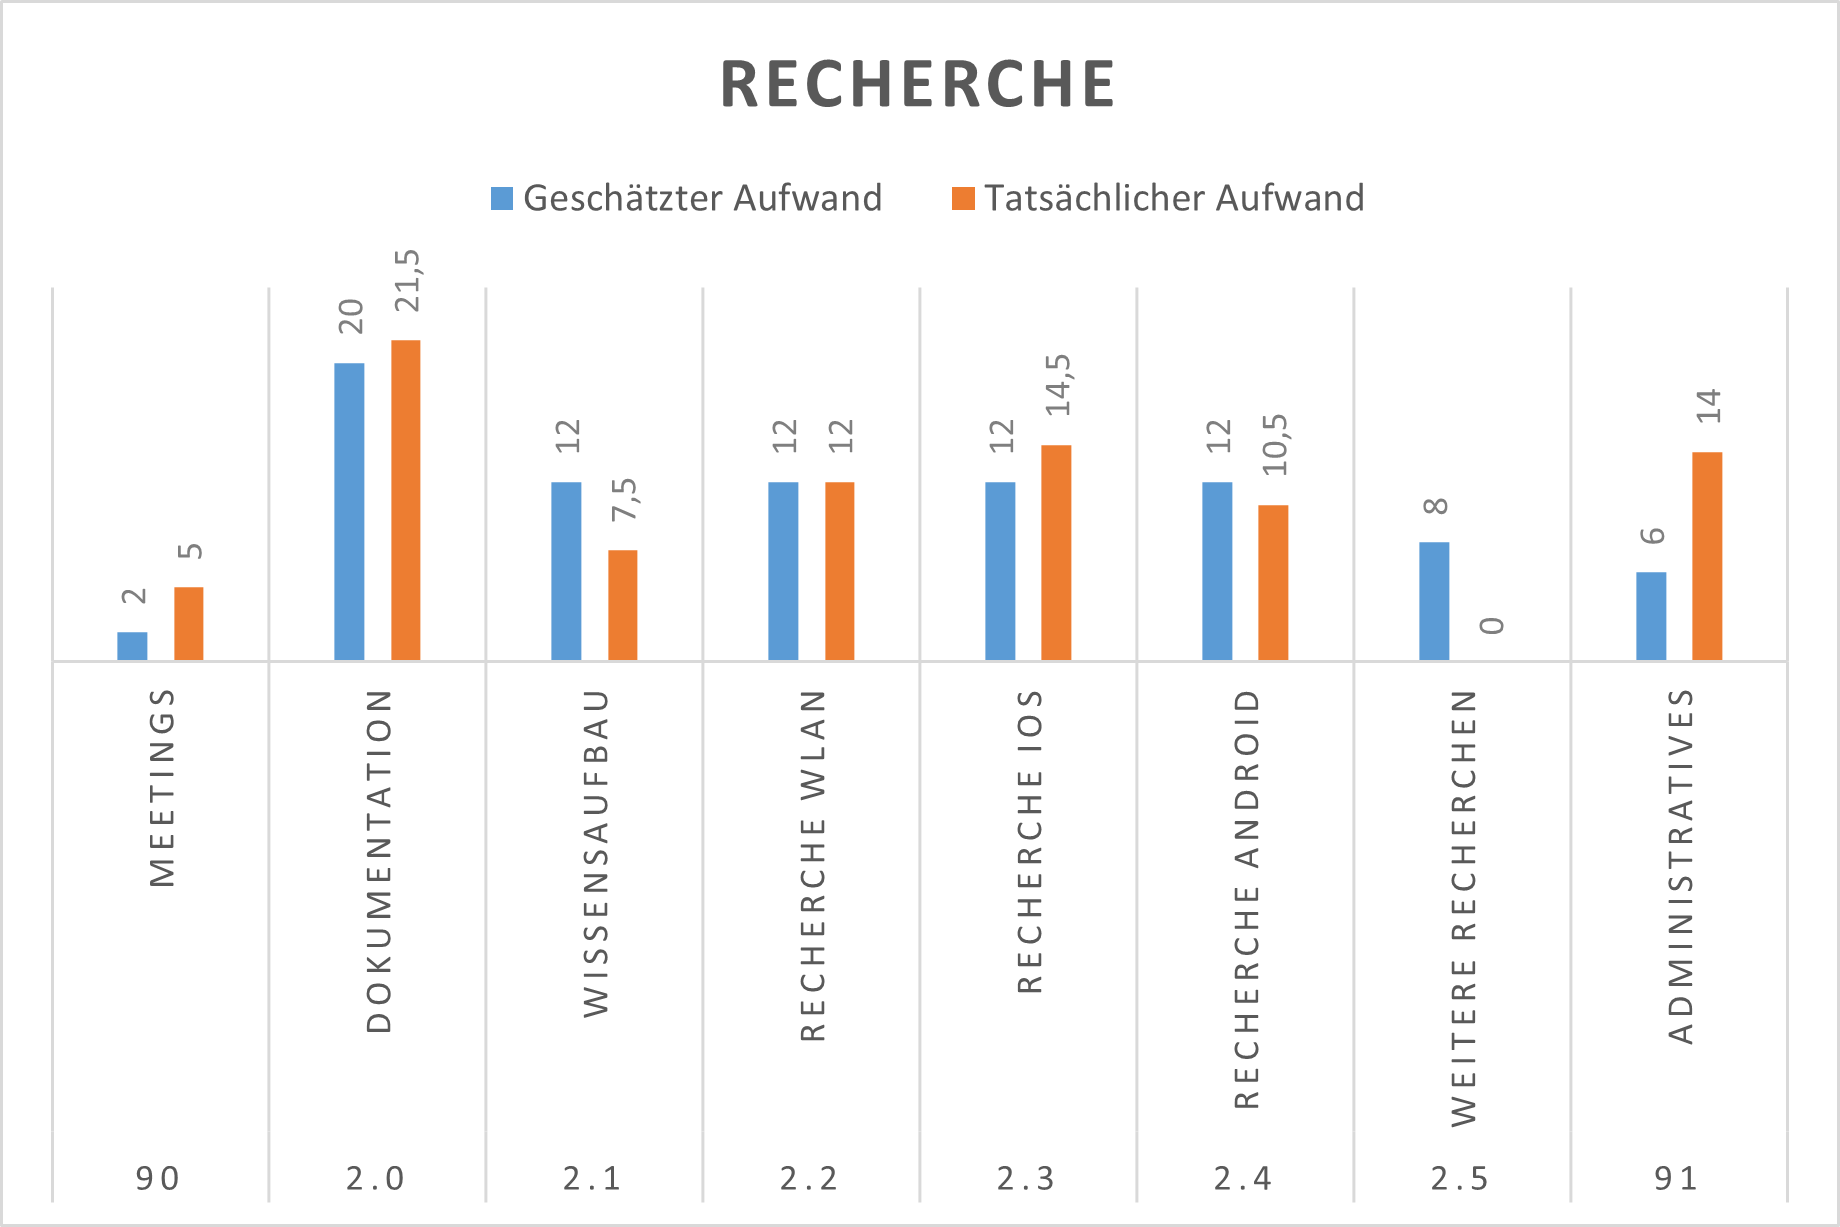
\includegraphics[width=1\linewidth]{Projectmanagement/Recherche_Auswertung.png}
	\caption{Auswertung der Arbeitspakete in der Recherchephase
	\label{figure:researchevaluation}}
\end{figure}

Geplanter Aufwand: $84$ Stunden. \\
Tatsächlicher Aufwand: $85$ Stunden.

Die weiteren Recherchen wurden als Reserve eingeplant, falls sich 
die Projektteilnehmer für die dritte Phase noch zusätzlich in eine Technologie
einarbeiten müssten. 

Vor allem der administrative Aufwand wurde unterschätzt. 
Die Beschaffung der benötigten Mobilgeräte hat mehr Zeit beansprucht, als 
ursprünglich angenommen.  

\clearpage

\subsubsection*{Phase 3: Experimente, Evaluierung und Prototyp}
\begin{figure}[h!]
	\centering
	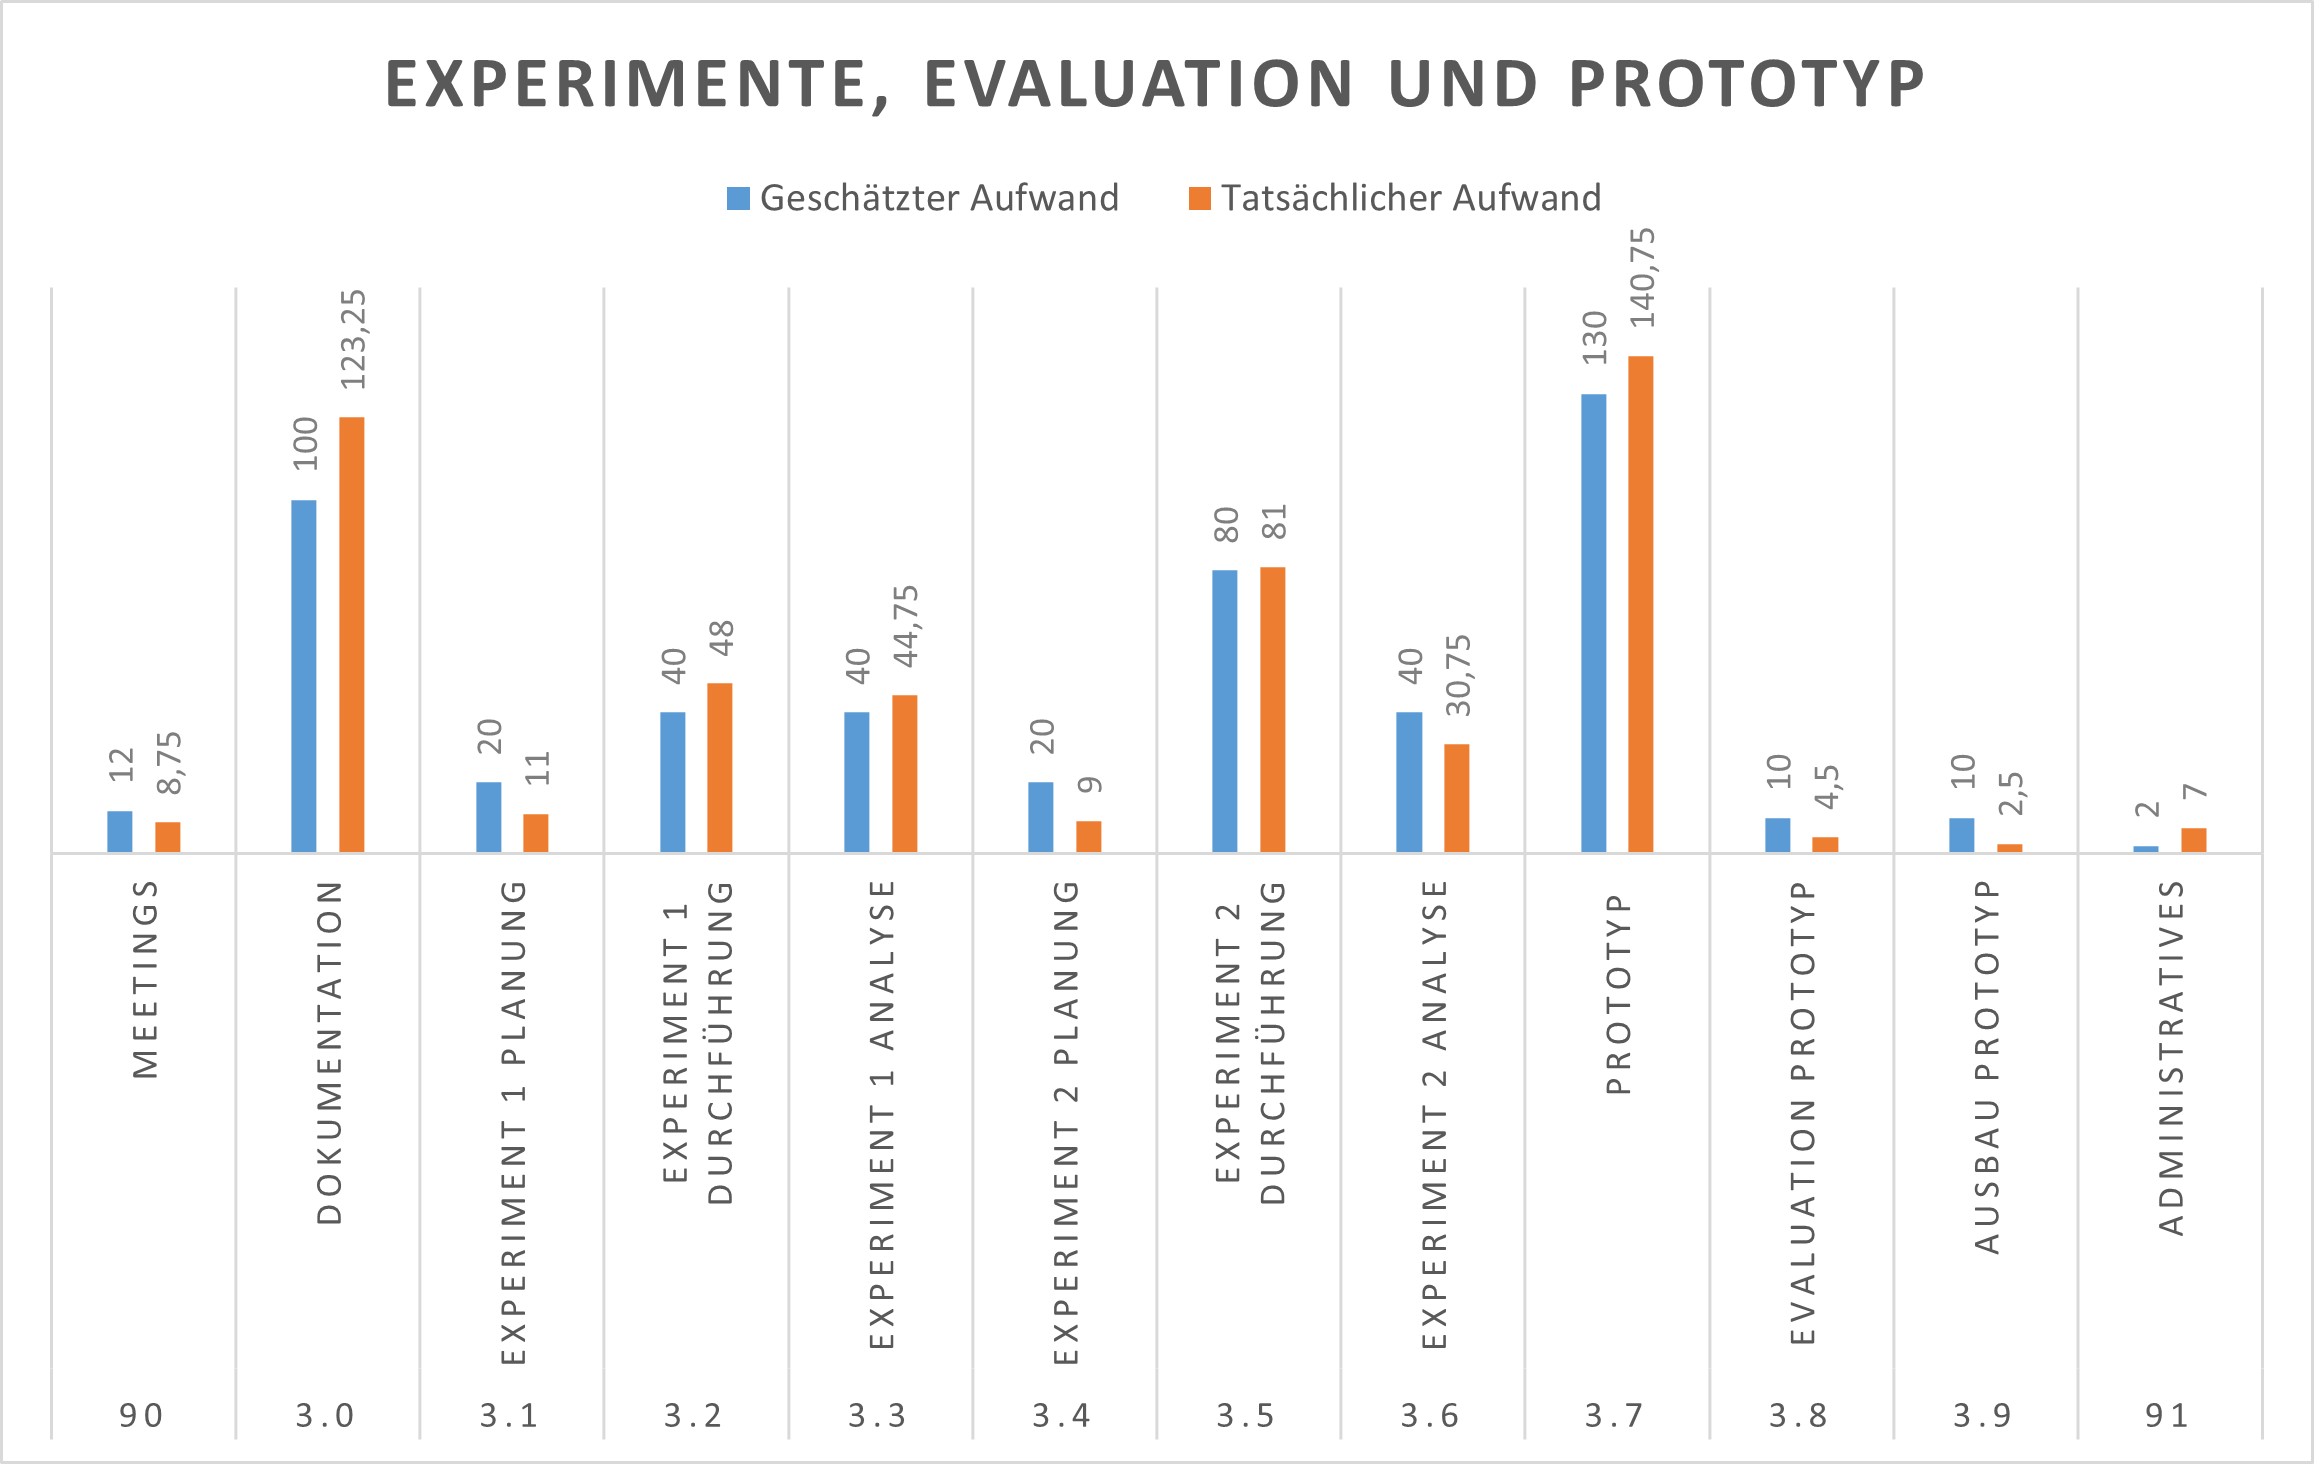
\includegraphics[width=1\linewidth]{Projectmanagement/EEP_Auswertung.png}
	\caption{Auswertung der Arbeitspakete in der dritten Phase
	\label{figure:eepevaluation}}
\end{figure}

Geplanter Aufwand: $504$ Stunden. \\
Tatsächlicher Aufwand: $511.25$ Stunden.

In der dritten Phase hatte es im Verlauf der Arbeit eine Änderung in der Planung 
gegeben. Die Android Messungen benötigten mehr Zeit als die iOS-Messungen. 
Im Meeting der Woche 7 wurde besprochen, dass die Messungen der Android-Geräte 
um eine Woche verlängert werden. Dadurch wurde die geschätzte Zeit für das 
Arbeitspaket von $40$ auf $80$ Stunden erhöht. Die Zeit wurde von den 
Arbeitspaketen Experiment 1 \& 2 Planung 
(zuvor je $40$ Stunden, danach $20$ Stunden) entfernt.

Vor allem die Arbeitspakete Dokumentation und Prototyp haben mehr Zeit 
beansprucht, als ursprünglich geplant. 

\clearpage 

\subsubsection*{Phase 4: Abschluss}
\begin{figure}[h!]
	\centering
	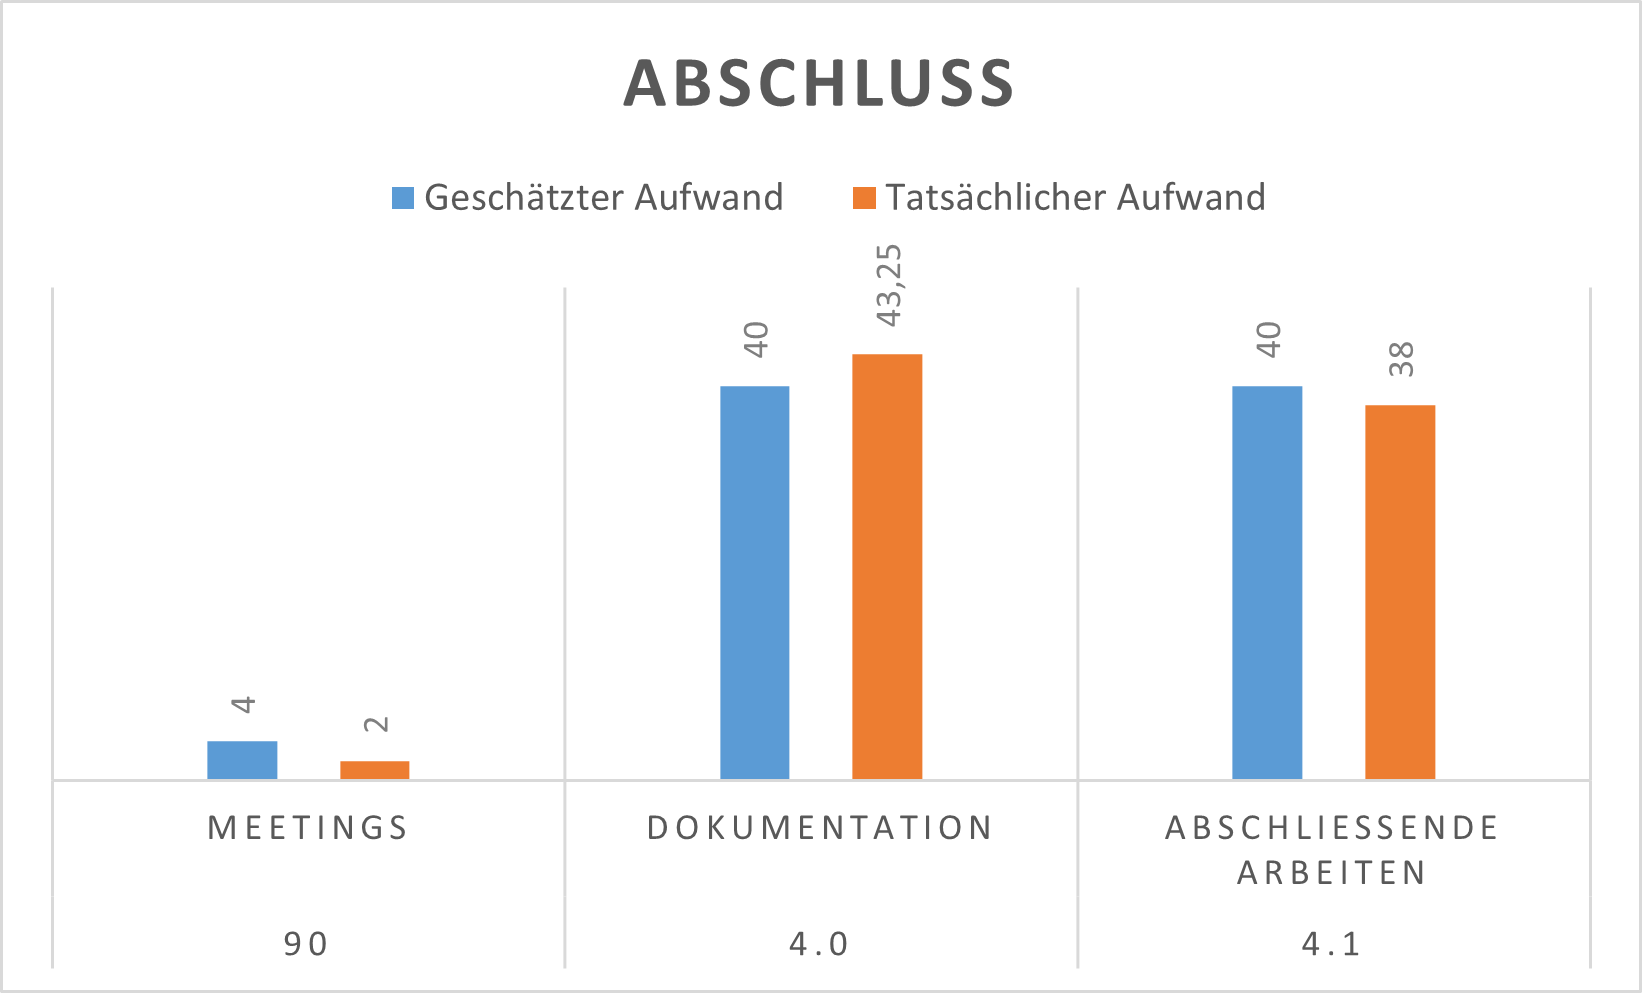
\includegraphics[width=1\linewidth]{Projectmanagement/Abschluss_Auswertung.png}
	\caption{Auswertung der Arbeitspakete in der Abschlussphase
	\label{figure:finishevaluation}}
\end{figure}

Geplanter Aufwand: $84$ Stunden. \\
Tatsächlicher Aufwand: $83.25$ Stunden.

\clearpage

\section{Infrastruktur 
\label{Infrastruktur}}
Beide Projektmitarbeiter verwenden ihre eigenen Notebooks mit Windows 10 
für die Durchführung der Bachelorarbeit. 
Weitere Hardware, die im Verlauf der Arbeit verwendet wird, 
wird fortlaufend dokumentiert.

\subsection*{Übersicht der Tools}
\begin{table}[H]
	\centering
	\begin{tabularx}{\linewidth}{l X}
		\toprule 
		\textbf{Bezeichnung} & \textbf{Verwendungsgrund} \\
		\midrule
		GitHub & Versionsverwaltung und Continuous Integration/Delivery \\
		GitKraken / SourceTree & Graphische Benutzeroberfläche für Git-Verwaltung \\
		Latex \& Visual Studio Code & Verfassung der Dokumentation \\
		Microsoft Excel & Zeiterfassung, Arbeitspakete und Spreadsheet-Auswertungen \\
		Whatsapp / Discord & Kommunikation innerhalb des Teams \\
		Microsoft Teams & Kommunikation mit dem Betreuer \\
		\bottomrule 
	\end{tabularx} 
	\caption{Übersicht der Tools
	\label{table:UebersichtTools}} 
\end{table}

\subsection*{Im Verlauf der Arbeit hinzugezogene Tools}
\begin{table}[H]
	\centering
	\begin{tabularx}{\linewidth}{l X}
		\toprule 
		\textbf{Bezeichnung} & \textbf{Verwendungsgrund} \\
		\midrule
		Wireshark & Messungen der Mobilgeräte \\
		\midrule
		Pycharm & Python Entwicklungsumgebung \\
		\bottomrule 
	\end{tabularx} 
	\caption{Hinzugezogene Tools
	\label{table:HinzugezogeneTools}} 
\end{table}

\clearpage 

\subsection*{Verwendete Hardware}
Die Tabelle~\ref{table:VerwendeteHardware} zeigt die in den Experimenten und
Prototypenentwicklung verwendete Hardware, den Gerätetypen und
den Hersteller. Mobilgeräte für die Messungen sind in den jeweiligen Abschnitten 
dokumentiert (iOS: Abschnitt~\ref{section:iosmeasurements} 
Tabelle~\ref{table:measurediosdevices}. 
Android: Abschnitt~\ref{section:androidmeasurements} 
Tabelle~\ref{table:measuredandroiddevices})
\begin{table}[H]
	\centering
	\begin{tabularx}{\linewidth}{l l l}
		\toprule 
		\textbf{Gerätebezeichnung} & \textbf{Gerätetyp} & \textbf{Hersteller} \\
		\midrule
		CAT S60 & Smartphone & Bullit Group \\
		\midrule 
		Macbook Pro & Laptop & Apple \\
		\midrule 
		WaveXpert & WLAN-Messgerät & Softing IT Networks GmbH  \\
		\bottomrule 
	\end{tabularx} 
	\caption{Verwendete Hardware
	\label{table:VerwendeteHardware}} 
\end{table}

\clearpage

\section{Qualitätsmassnahmen
\label{Qualitätsmassnahmen}}
Um für die Bachelorarbeit die Qualität zu gewährleisten, 
werden folgende Massnahmen getroffen:

\subsection*{Dokumentation}
Damit die Dokumentation über die Versionsverwaltung gemeinsam von allen 
Projektteilnehmern vorgenommen werden kann, wird ein Latex-Dokument 
aufgesetzt und über GitHub verwaltet.

\subsection*{Projektmanagement}
\subsubsection*{GitHub}
Für die Versionsverwaltung wird ein GitHub-Repository aufgesetzt. 
Im Bedarfsfall wird für die Umsetzung eines Prototyps eine Continuous 
Integration / Continuous Delivery Pipeline und allenfalls weitere 
Hilfsfunktionen konfiguriert.

Der main- und development-Branch sind beide so abgesichert, 
dass kein Projektteilnehmer direkt seine Änderung darauf Pushen kann, 
sondern die Anpassungen über einen Pull-Request eingibt. 
Dieser Request wird vom jeweils anderen Projektpartner kontrolliert 
und akzeptiert oder abgelehnt. Die Projektmitglieder verwenden für die 
Implementation jeweils spezifische Feature-Branches.

Diese Arbeitsweise erlaubt es, einen sicheren Arbeitsfluss zu gewährleisten, 
bei dem wenig Merge-Konflikte auftreten sollten und bei dem jede Änderung 
zuerst vom Partner durch ein Review abgesegnet werden muss, 
bevor sie integriert wird.

\subsubsection*{Prozessmodell}
Die Bachelorarbeit als Ganzes wird als Wasserfall-Modell aufgezogen. 
Der Beginn und das Ende der Arbeit sowie drei der Vier Projektphasen 
sind klar spezifiziert. 
Lediglich die dritte Phase wird als Iterative Phase durchgeführt, 
da im Vornherein nicht gesagt werden kann,
welche Resultate aus den Experimenten tatsächlich gewonnen werden können 
und ob diese Resultate für die Entwicklung eines Prototyps verwendet werden
können.

\clearpage 

\subsubsection*{Experimenteller Aufbau}
Damit die Experimente mit möglichst signifikanten Ergebnissen ausgeführt 
werden können, muss vor jeder Durchführung ein Plan mit den Parametern 
erstellt werden, wie genau das Experiment unter welchen Bedingungen 
durchgeführt wird, wie die zu erwartenden Ergebnisse aussehen und welche
Daten für die weitere Verwendung in welchem Format gespeichert werden sollen.
Nach den Experimenten müssen die Ergebnisse ausgewertet und dokumentiert werden. 